% 2018 江苏卷第10题：正方体中心多面体（正八面体）
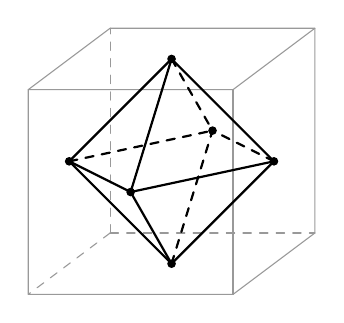
\begin{tikzpicture}[font=\small, line cap=round, line join=round, >=stealth, scale=1.3]
  % 正方体顶点
  \coordinate (A) at (0, 0);
  \coordinate (B) at (2, 0);
  \coordinate (C) at (2.8, 0.6);
  \coordinate (D) at (0.8, 0.6);
  \coordinate (A1) at (0, 2);
  \coordinate (B1) at (2, 2);
  \coordinate (C1) at (2.8, 2.6);
  \coordinate (D1) at (0.8, 2.6);

  % 六个面中心
  \coordinate (F_front) at (1, 1);
  \coordinate (F_back) at (1.8, 1.6);
  \coordinate (F_left) at (0.4, 1.3);
  \coordinate (F_right) at (2.4, 1.3);
  \coordinate (F_bottom) at (1.4, 0.3);
  \coordinate (F_top) at (1.4, 2.3);

  % 正方体虚线棱
  \draw[dashed, thin, gray!80] (D) -- (A);
  \draw[dashed, thin, gray!80] (D) -- (C);
  \draw[dashed, thin, gray!80] (D) -- (D1);

  % 正方体实线棱
  \draw[thin, gray!80] (A) -- (B) -- (C) -- (C1) -- (D1) -- (A1) -- cycle;
  \draw[thin, gray!80] (B) -- (B1);
  \draw[thin, gray!80] (A1) -- (B1) -- (C1);

  % 多面体虚线棱（连接后部和内部的中心）
  \draw[dashed, thick] (F_top) -- (F_back);
  \draw[dashed, thick] (F_bottom) -- (F_back);
  \draw[dashed, thick] (F_left) -- (F_back);
  \draw[dashed, thick] (F_right) -- (F_back);

  % 多面体实线棱
  \draw[thick] (F_top) -- (F_front);
  \draw[thick] (F_top) -- (F_left);
  \draw[thick] (F_top) -- (F_right);
  \draw[thick] (F_bottom) -- (F_front);
  \draw[thick] (F_bottom) -- (F_left);
  \draw[thick] (F_bottom) -- (F_right);
  \draw[thick] (F_front) -- (F_left);
  \draw[thick] (F_front) -- (F_right);

  % 各中心点标记
  \foreach \p in {F_front, F_back, F_left, F_right, F_bottom, F_top} {
    \fill (\p) circle (1.2pt);
  }
\end{tikzpicture}
